% Options for packages loaded elsewhere
\PassOptionsToPackage{unicode}{hyperref}
\PassOptionsToPackage{hyphens}{url}
%
\documentclass[
  a4paper]{article}
\usepackage{lmodern}
\usepackage{amssymb,amsmath}
\usepackage{ifxetex,ifluatex}
\ifnum 0\ifxetex 1\fi\ifluatex 1\fi=0 % if pdftex
  \usepackage[T1]{fontenc}
  \usepackage[utf8]{inputenc}
  \usepackage{textcomp} % provide euro and other symbols
\else % if luatex or xetex
  \usepackage{unicode-math}
  \defaultfontfeatures{Scale=MatchLowercase}
  \defaultfontfeatures[\rmfamily]{Ligatures=TeX,Scale=1}
  \setsansfont[]{Calibri Light}
\fi
% Use upquote if available, for straight quotes in verbatim environments
\IfFileExists{upquote.sty}{\usepackage{upquote}}{}
\IfFileExists{microtype.sty}{% use microtype if available
  \usepackage[]{microtype}
  \UseMicrotypeSet[protrusion]{basicmath} % disable protrusion for tt fonts
}{}
\makeatletter
\@ifundefined{KOMAClassName}{% if non-KOMA class
  \IfFileExists{parskip.sty}{%
    \usepackage{parskip}
  }{% else
    \setlength{\parindent}{0pt}
    \setlength{\parskip}{6pt plus 2pt minus 1pt}}
}{% if KOMA class
  \KOMAoptions{parskip=half}}
\makeatother
\usepackage{xcolor}
\IfFileExists{xurl.sty}{\usepackage{xurl}}{} % add URL line breaks if available
\IfFileExists{bookmark.sty}{\usepackage{bookmark}}{\usepackage{hyperref}}
\hypersetup{
  hidelinks,
  pdfcreator={LaTeX via pandoc}}
\urlstyle{same} % disable monospaced font for URLs
\usepackage[margin=1in]{geometry}
\usepackage{graphicx,grffile}
\makeatletter
\def\maxwidth{\ifdim\Gin@nat@width>\linewidth\linewidth\else\Gin@nat@width\fi}
\def\maxheight{\ifdim\Gin@nat@height>\textheight\textheight\else\Gin@nat@height\fi}
\makeatother
% Scale images if necessary, so that they will not overflow the page
% margins by default, and it is still possible to overwrite the defaults
% using explicit options in \includegraphics[width, height, ...]{}
\setkeys{Gin}{width=\maxwidth,height=\maxheight,keepaspectratio}
% Set default figure placement to htbp
\makeatletter
\def\fps@figure{htbp}
\makeatother
\setlength{\emergencystretch}{3em} % prevent overfull lines
\providecommand{\tightlist}{%
  \setlength{\itemsep}{0pt}\setlength{\parskip}{0pt}}
\setcounter{secnumdepth}{-\maxdimen} % remove section numbering
\usepackage{fancyhdr}
\usepackage[T1]{fontenc}
\usepackage[default]{sourcesanspro}
\usepackage{tikz}
\addtolength{\headheight}{1.0cm} 
\fancypagestyle{plain}{} 
\thispagestyle{fancy} 
\renewcommand{\headrulewidth}{0pt}

% Package for references with numbers
\bibliographystyle{apsrev4-1}
\usepackage[numbers]{natbib}
\setcitestyle{numbers}
\usepackage[brazil]{babel}
\usepackage{amsmath}
\usepackage{titling}

\usepackage{background}

\backgroundsetup{
position={3,0.55},
scale=1.2,
color=black,
opacity=1,
angle=0,
pages=all,
contents={%
  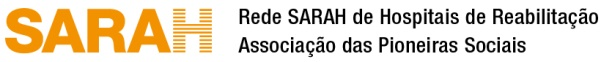
\includegraphics[width=200px,height=200px]{Imagens/logo_header.jpg}
  }%
}
\usepackage{floatrow}
\floatsetup[figure]{capposition=top}
\floatsetup[table]{capposition=top}


\usepackage{fancyhdr}
\pagestyle{fancy}
% center of header
\fancyhf{} % clear all header and footer fields

\renewcommand{\headrulewidth}{0pt}
\usepackage{booktabs}
\usepackage{longtable}
\usepackage{array}
\usepackage{multirow}
\usepackage{wrapfig}
\usepackage{float}
\usepackage{colortbl}
\usepackage{pdflscape}
\usepackage{tabu}
\usepackage{threeparttable}
\usepackage{threeparttablex}
\usepackage[normalem]{ulem}
\usepackage{makecell}
\usepackage{xcolor}

\author{}
\date{\vspace{-2.5em}}

\begin{document}

\rhead{\fontsize{8pt}{10pt} \selectfont Núcleo de Segurança do Paciente
\\ \fontsize{8pt}{10pt} \selectfont Centro Nacional de Controle de Qualidade
\\ \fontsize{8pt}{10pt} \selectfont 1°Estágio – Relatório de Notificações
}

\section{NOTIFICAÇÕES – Ano 2021, 1º Estágio}

\subsection{Queda}

\begin{table}[H]

\caption{\label{tab:unnamed-chunk-3}Distribuição das quedas mês a mês de acordo com o dano.}
\centering
\resizebox{\linewidth}{!}{
\begin{tabular}[t]{lrrrrrrrrrrrr}
\toprule
 & jan & fev & mar & abr & mai & jun & jul & ago & set & out & nov & Total\\
\midrule
Incidente sem dano & 0 & 1 & 0 & 0 & 0 & 0 & 0 & 1 & 0 & 0 & 0 & 2\\
\midrule
\textbf{Total} & \textbf{0} & \textbf{1} & \textbf{0} & \textbf{0} & \textbf{0} & \textbf{0} & \textbf{0} & \textbf{1} & \textbf{0} & \textbf{0} & \textbf{0} & \textbf{2}\\
\bottomrule
\end{tabular}}
\end{table}

\begin{figure}[H]
\caption{Distribuição da queda de acordo com o período.}
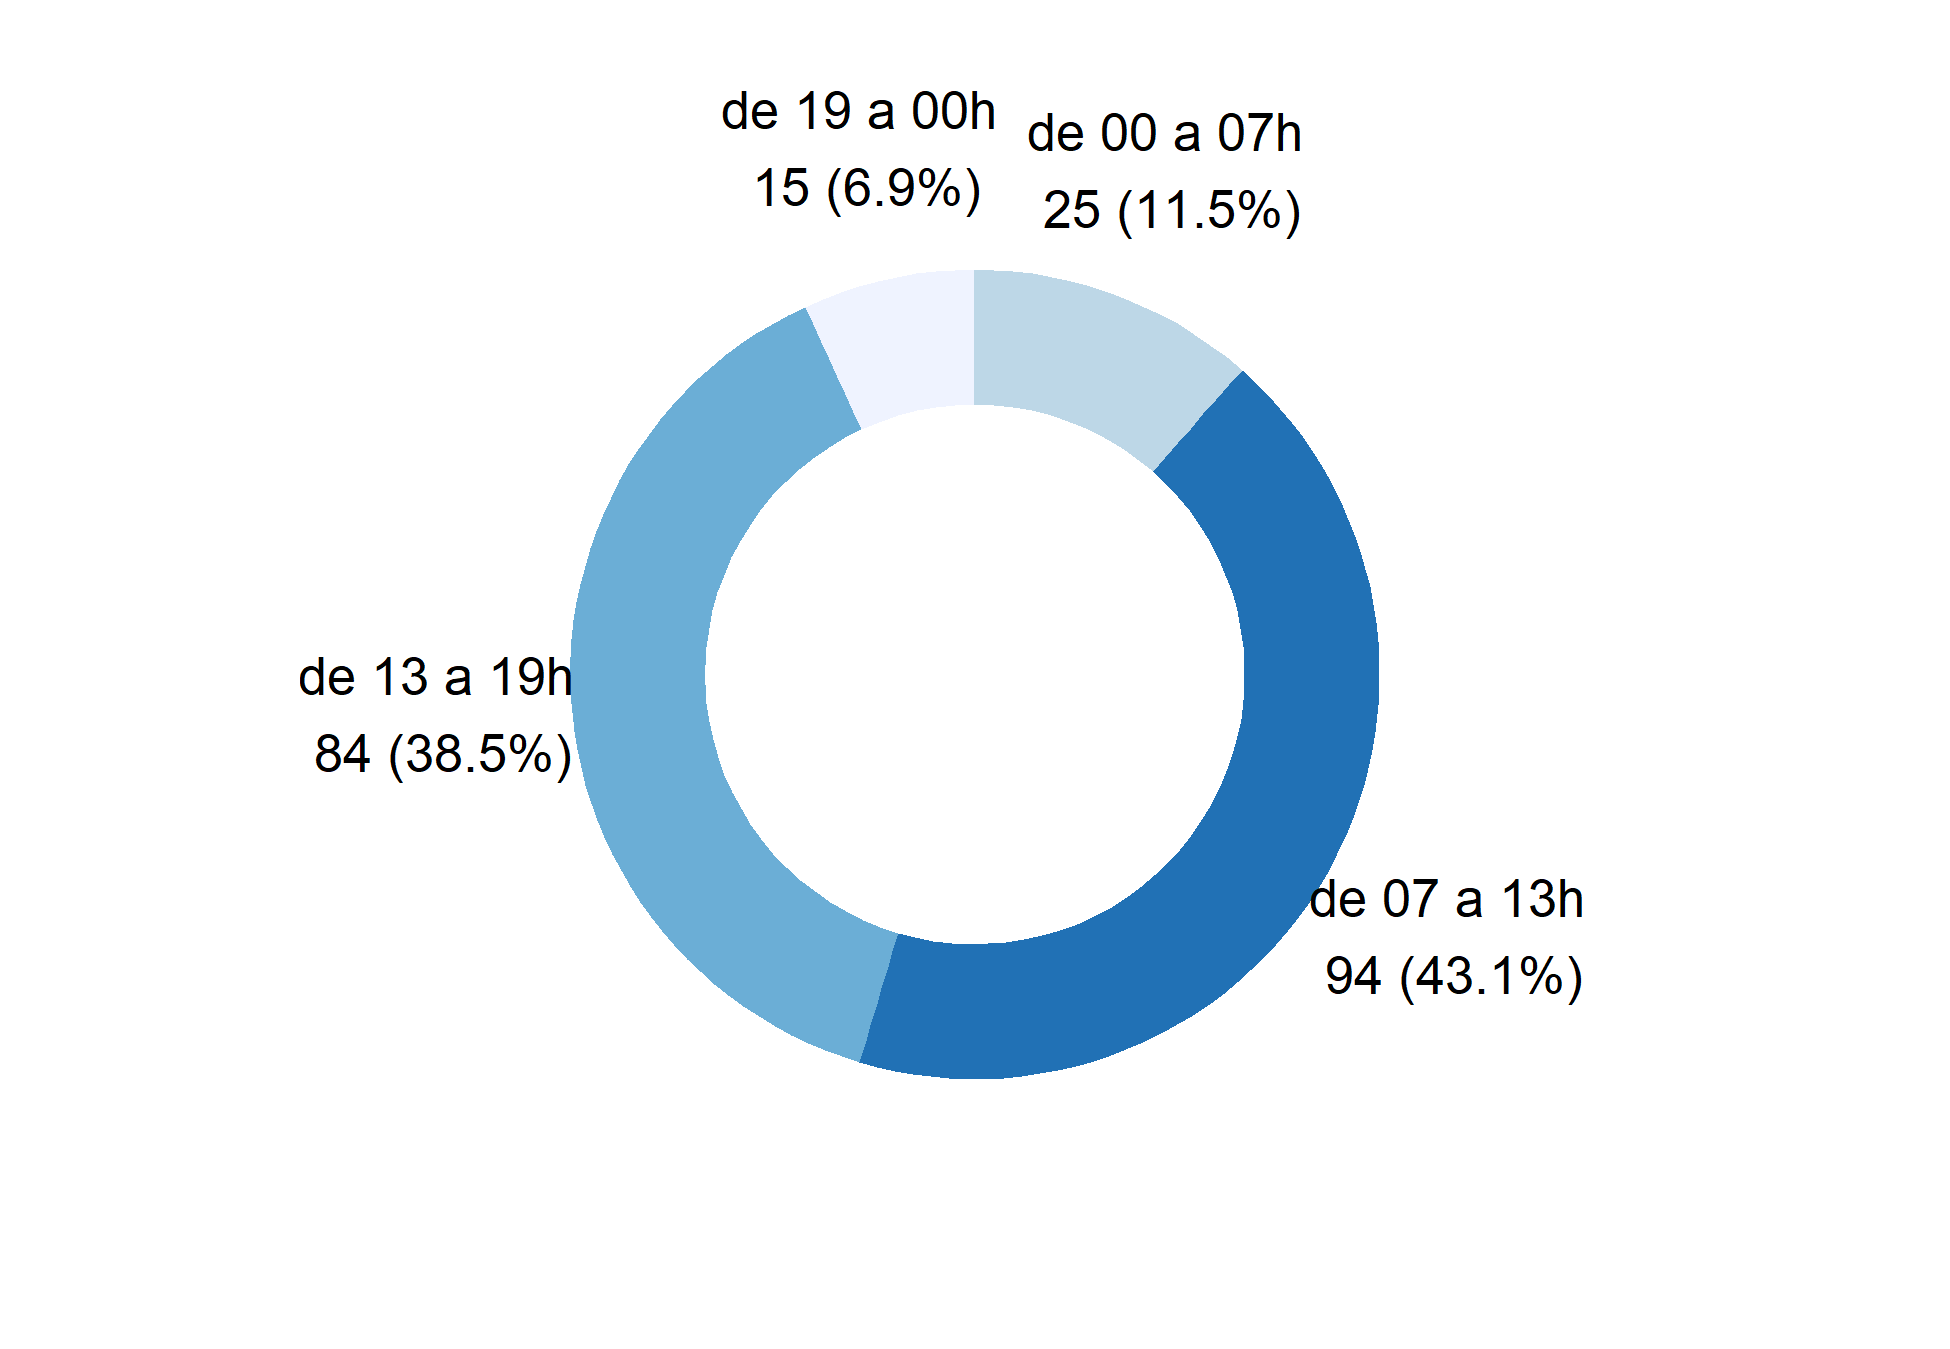
\includegraphics[width=0.7\textwidth]{Imagens/queda_periodo.png}
\end{figure}

\begin{table}[H]

\caption{\label{tab:unnamed-chunk-5}Motivo da queda.}
\centering
\begin{tabular}[t]{lr}
\toprule
Motivo da Queda & Total\\
\midrule
Outros & 1\\
Síncope & 1\\
\midrule
\textbf{Total} & \textbf{2}\\
\bottomrule
\end{tabular}
\end{table}

\begin{table}[H]

\caption{\label{tab:unnamed-chunk-6}Atividade durante a queda.}
\centering
\begin{tabular}[t]{lr}
\toprule
Atividade & Total\\
\midrule
Higiene & 1\\
Sono/Repouso & 1\\
\midrule
\textbf{Total} & \textbf{2}\\
\bottomrule
\end{tabular}
\end{table}

\newpage

\begin{table}[H]

\caption{\label{tab:unnamed-chunk-7}Superfície envolvida na queda.}
\centering
\begin{tabular}[t]{lr}
\toprule
Superfície & Total\\
\midrule
Cama-maca & 1\\
Própria altura & 1\\
\midrule
\textbf{Total} & \textbf{2}\\
\bottomrule
\end{tabular}
\end{table}

\begin{figure}[H]
\caption{Presença de acompanhante no momento da queda.}
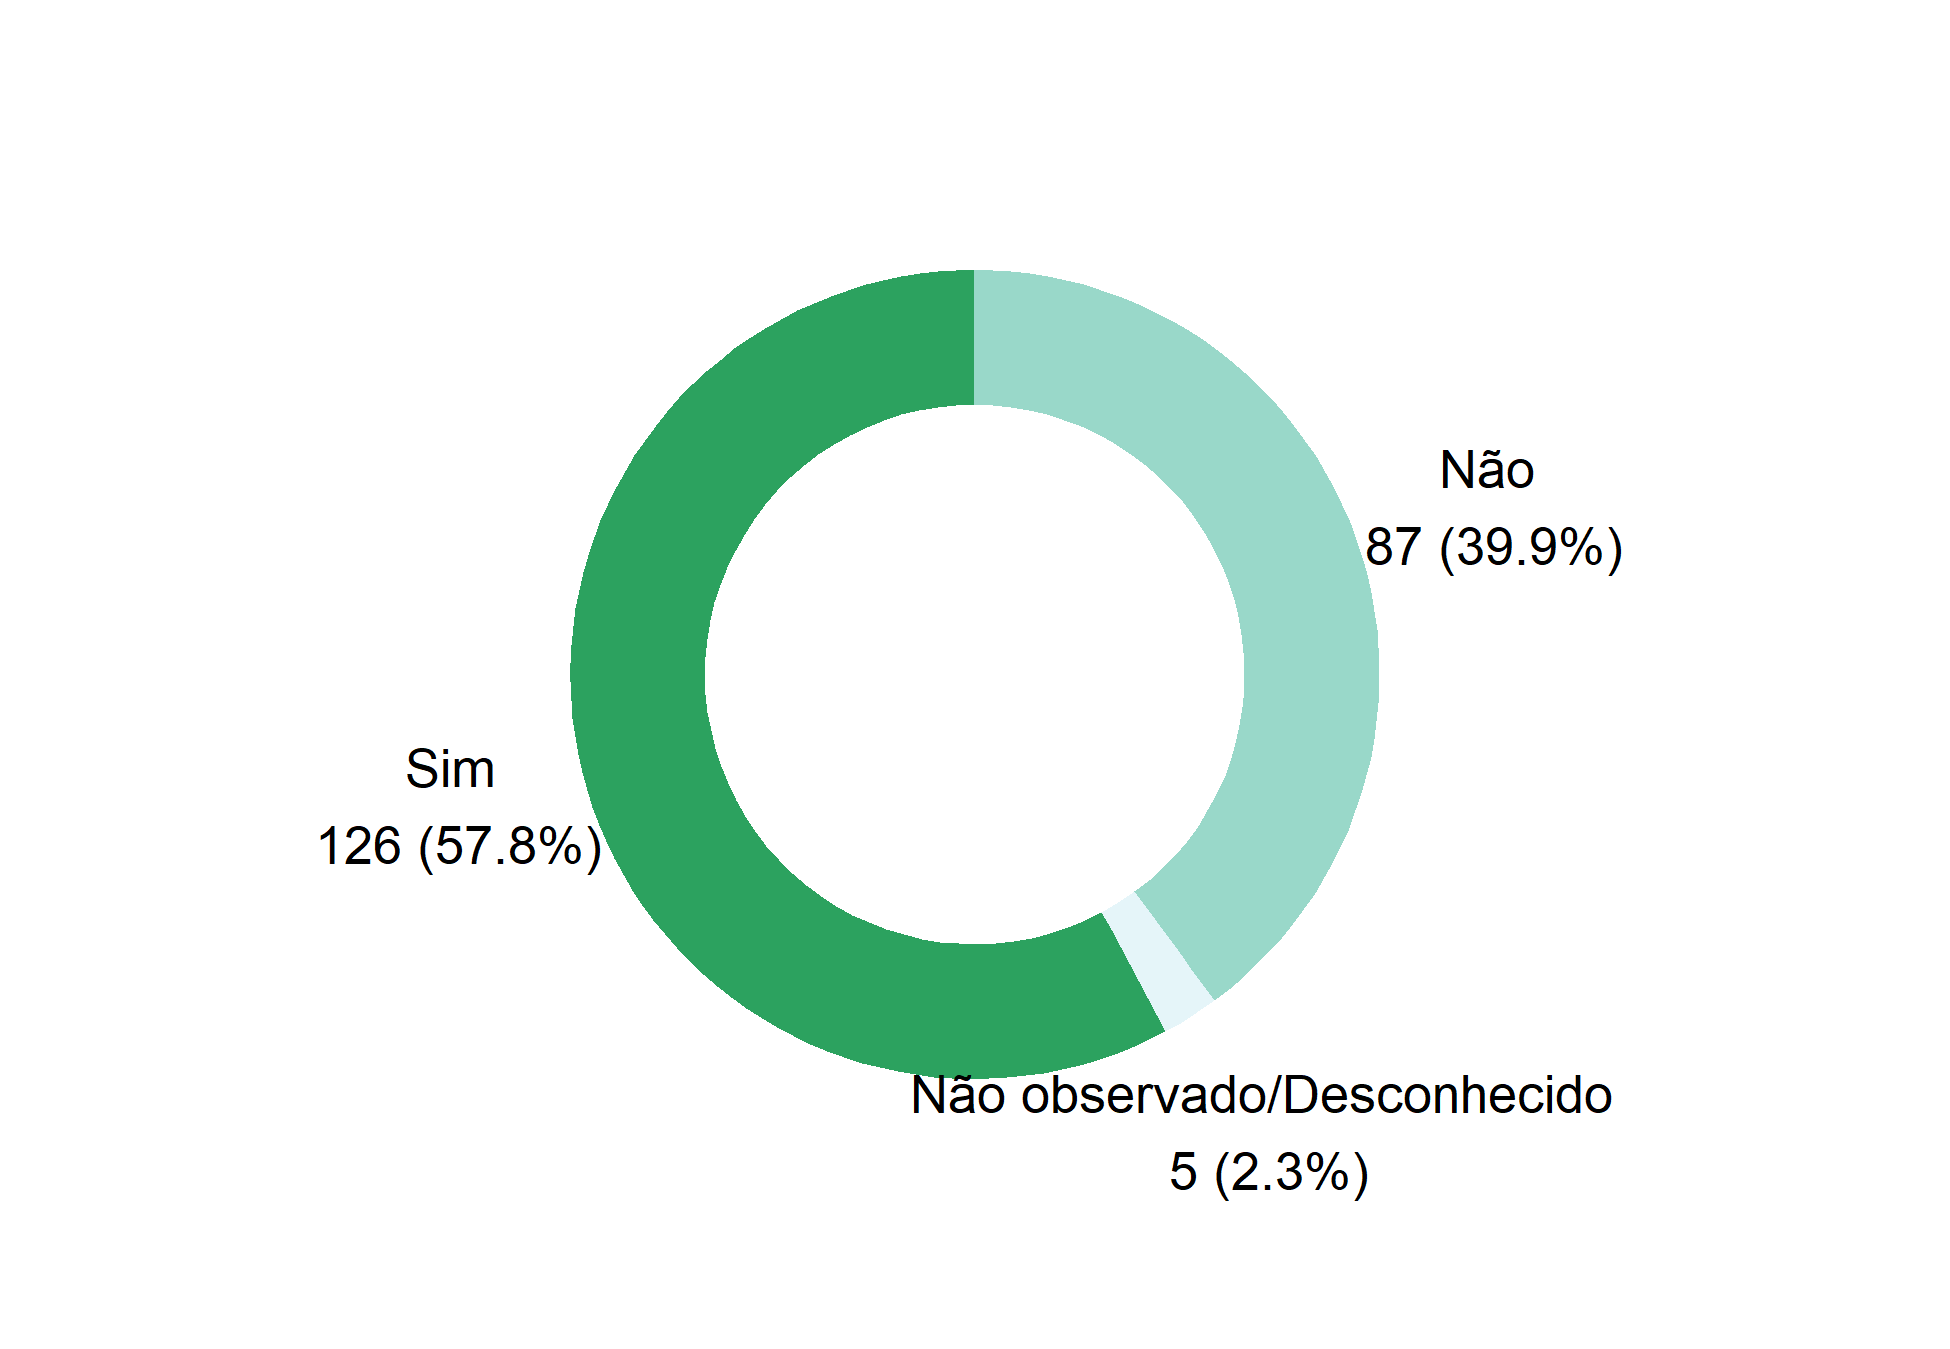
\includegraphics[width=0.7\textwidth]{Imagens/queda_acomp.png}
\end{figure}

\newpage

\subsection{Lesão por Pressão (LP)}

\begin{table}[H]

\caption{\label{tab:unnamed-chunk-9}Tipo de Lesão por Pressão.}
\centering
\resizebox{\linewidth}{!}{
\begin{tabular}[t]{lrrrrrrrrrrrr}
\toprule
 & jan & fev & mar & abr & mai & jun & jul & ago & set & out & nov & Total\\
\midrule
Em membranas mucosas & 0 & 0 & 0 & 0 & 0 & 0 & 1 & 0 & 0 & 0 & 0 & 1\\
Em proeminências ósseas & 1 & 0 & 1 & 0 & 0 & 0 & 0 & 1 & 1 & 0 & 0 & 4\\
Relacionada a dispositivo médico & 0 & 0 & 1 & 1 & 0 & 1 & 0 & 4 & 0 & 0 & 0 & 7\\
\midrule
\textbf{Total} & \textbf{1} & \textbf{0} & \textbf{2} & \textbf{1} & \textbf{0} & \textbf{1} & \textbf{1} & \textbf{5} & \textbf{1} & \textbf{0} & \textbf{0} & \textbf{12}\\
\bottomrule
\end{tabular}}
\end{table}

\subsubsection{Lesão por Pressão em Proeminência Óssea}

\hspace{1cm} Em 2020 houve uma LP estágio 1, no ísquio em paciente do
gênero masculino. A outra foi estágio 2, no pavilhão auditivo em
paciente do gênero feminino; ambas primárias.

\subsubsection{Lesão por Pressão Relacionada ao Dispositivo Médico}

\hspace{1cm} Em 2020, houve nove LP relacionadas ao Dispositivo Médico;
o comprometimento tissular está ilustrado abaixo:

\begin{table}[H]

\caption{\label{tab:unnamed-chunk-10}Comprometimento tissular na LP por dispositivo médico.}
\centering
\begin{tabular}[t]{lr}
\toprule
Comprometimento Tissular & Total\\
\midrule
Estágio 2 & 4\\
Estágio 1 & 2\\
Lesão tissular profunda & 1\\
\midrule
\textbf{Total} & \textbf{7}\\
\bottomrule
\end{tabular}
\end{table}

\begin{table}[H]

\caption{\label{tab:unnamed-chunk-11}Localização da LP por dispositivo médico.}
\centering
\begin{tabular}[t]{lr}
\toprule
Localização da LP & Total\\
\midrule
Corpo nasal & 2\\
Calcâneo & 1\\
coxa & 1\\
Flanco & 1\\
Projeção medial dos metatarsos & 1\\
\addlinespace
Zigomático & 1\\
\midrule
\textbf{Total} & \textbf{7}\\
\bottomrule
\end{tabular}
\end{table}

\subsection{Lesão Traumática}

\hspace{1cm} Em 2020 foi notificada uma lesão traumática do tipo abrasão
relacionada à procedimento cirúrgico.

\subsection{Lesão de Pele}

\hspace{1cm} Em 2020, foi notificada apenas duas lesões por adesivo, uma
delas com formação de flictena e outra com lesão de continuidade.

\subsubsection{Medicamento}

\begin{table}[H]

\caption{\label{tab:unnamed-chunk-12}Classificação das notificações em medicamentos.}
\centering
\resizebox{\linewidth}{!}{
\begin{tabular}[t]{lrrrrrrrrrrrr}
\toprule
 & jan & fev & mar & abr & mai & jun & jul & ago & set & out & nov & Total\\
\midrule
Evento Adverso & 0 & 0 & 0 & 1 & 0 & 0 & 0 & 3 & 3 & 2 & 1 & 10\\
Incidente sem dano & 3 & 1 & 0 & 2 & 4 & 6 & 1 & 5 & 4 & 2 & 2 & 30\\
Quase um erro (Near Miss) & 4 & 10 & 4 & 1 & 4 & 2 & 5 & 9 & 7 & 3 & 1 & 50\\
\midrule
\textbf{Total} & \textbf{7} & \textbf{11} & \textbf{4} & \textbf{4} & \textbf{8} & \textbf{8} & \textbf{6} & \textbf{17} & \textbf{14} & \textbf{7} & \textbf{4} & \textbf{90}\\
\bottomrule
\end{tabular}}
\end{table}

\begin{table}[H]

\caption{\label{tab:unnamed-chunk-13}Notificações no processo de prescrição de medicamentos.}
\centering
\begin{tabular}[t]{lr}
\toprule
Prescrição & Total\\
\midrule
Outros & 5\\
Dose incorreta & 4\\
Falta de medicamento & 4\\
Falta de frequência & 3\\
Duplicidade de medicamento & 1\\
\addlinespace
Falta da apresentação farmacêutica & 1\\
Falta de dose & 1\\
Forma farmacêutica ou apresentação incorreta & 1\\
Paciente incorreto & 1\\
Via de administração incorreta & 1\\
\midrule
\addlinespace
\textbf{Total} & \textbf{22}\\
\bottomrule
\end{tabular}
\end{table}

\begin{table}[H]

\caption{\label{tab:unnamed-chunk-14}Notificações no processo de dispensação de medicamentos.}
\centering
\begin{tabular}[t]{lr}
\toprule
Dispensação & Total\\
\midrule
Dose incorreta & 10\\
Medicamento incorreto & 8\\
Falta de medicamento & 5\\
Outros & 3\\
Medicamento com identificação incorreta/ausente & 2\\
\addlinespace
Dispensado e não encontrado & 1\\
Frequência incorreta & 1\\
Horário incorreto & 1\\
Paciente incorreto & 1\\
Via de administração incorreta & 1\\
\midrule
\addlinespace
\textbf{Total} & \textbf{33}\\
\bottomrule
\end{tabular}
\end{table}

\hspace{1cm} Não houve notificações de falhas na fase do preparo de
medicamentos no ano de 2020.

\begin{table}[H]

\caption{\label{tab:unnamed-chunk-15}Notificação no processo de administração de medicamentos.}
\centering
\begin{tabular}[t]{lr}
\toprule
Administração & Total\\
\midrule
Medicamento incorreto & 4\\
Medicamento não administrado (omissão) & 4\\
Outros & 4\\
Velocidade/Tempo de infusão incorreto & 4\\
Dose incorreta & 3\\
\addlinespace
Horário incorreto & 3\\
Ausência de registro/checagem & 2\\
Frequência incorreta & 1\\
Infiltração & 1\\
Paciente incorreto & 1\\
\midrule
\addlinespace
\textbf{Total} & \textbf{27}\\
\bottomrule
\end{tabular}
\end{table}

\subsection{Procedimento Cirúrgico}

\begin{figure}[H]
\caption{Distribuição do gênero nas notificações em Procedimento Cirúrgico.}
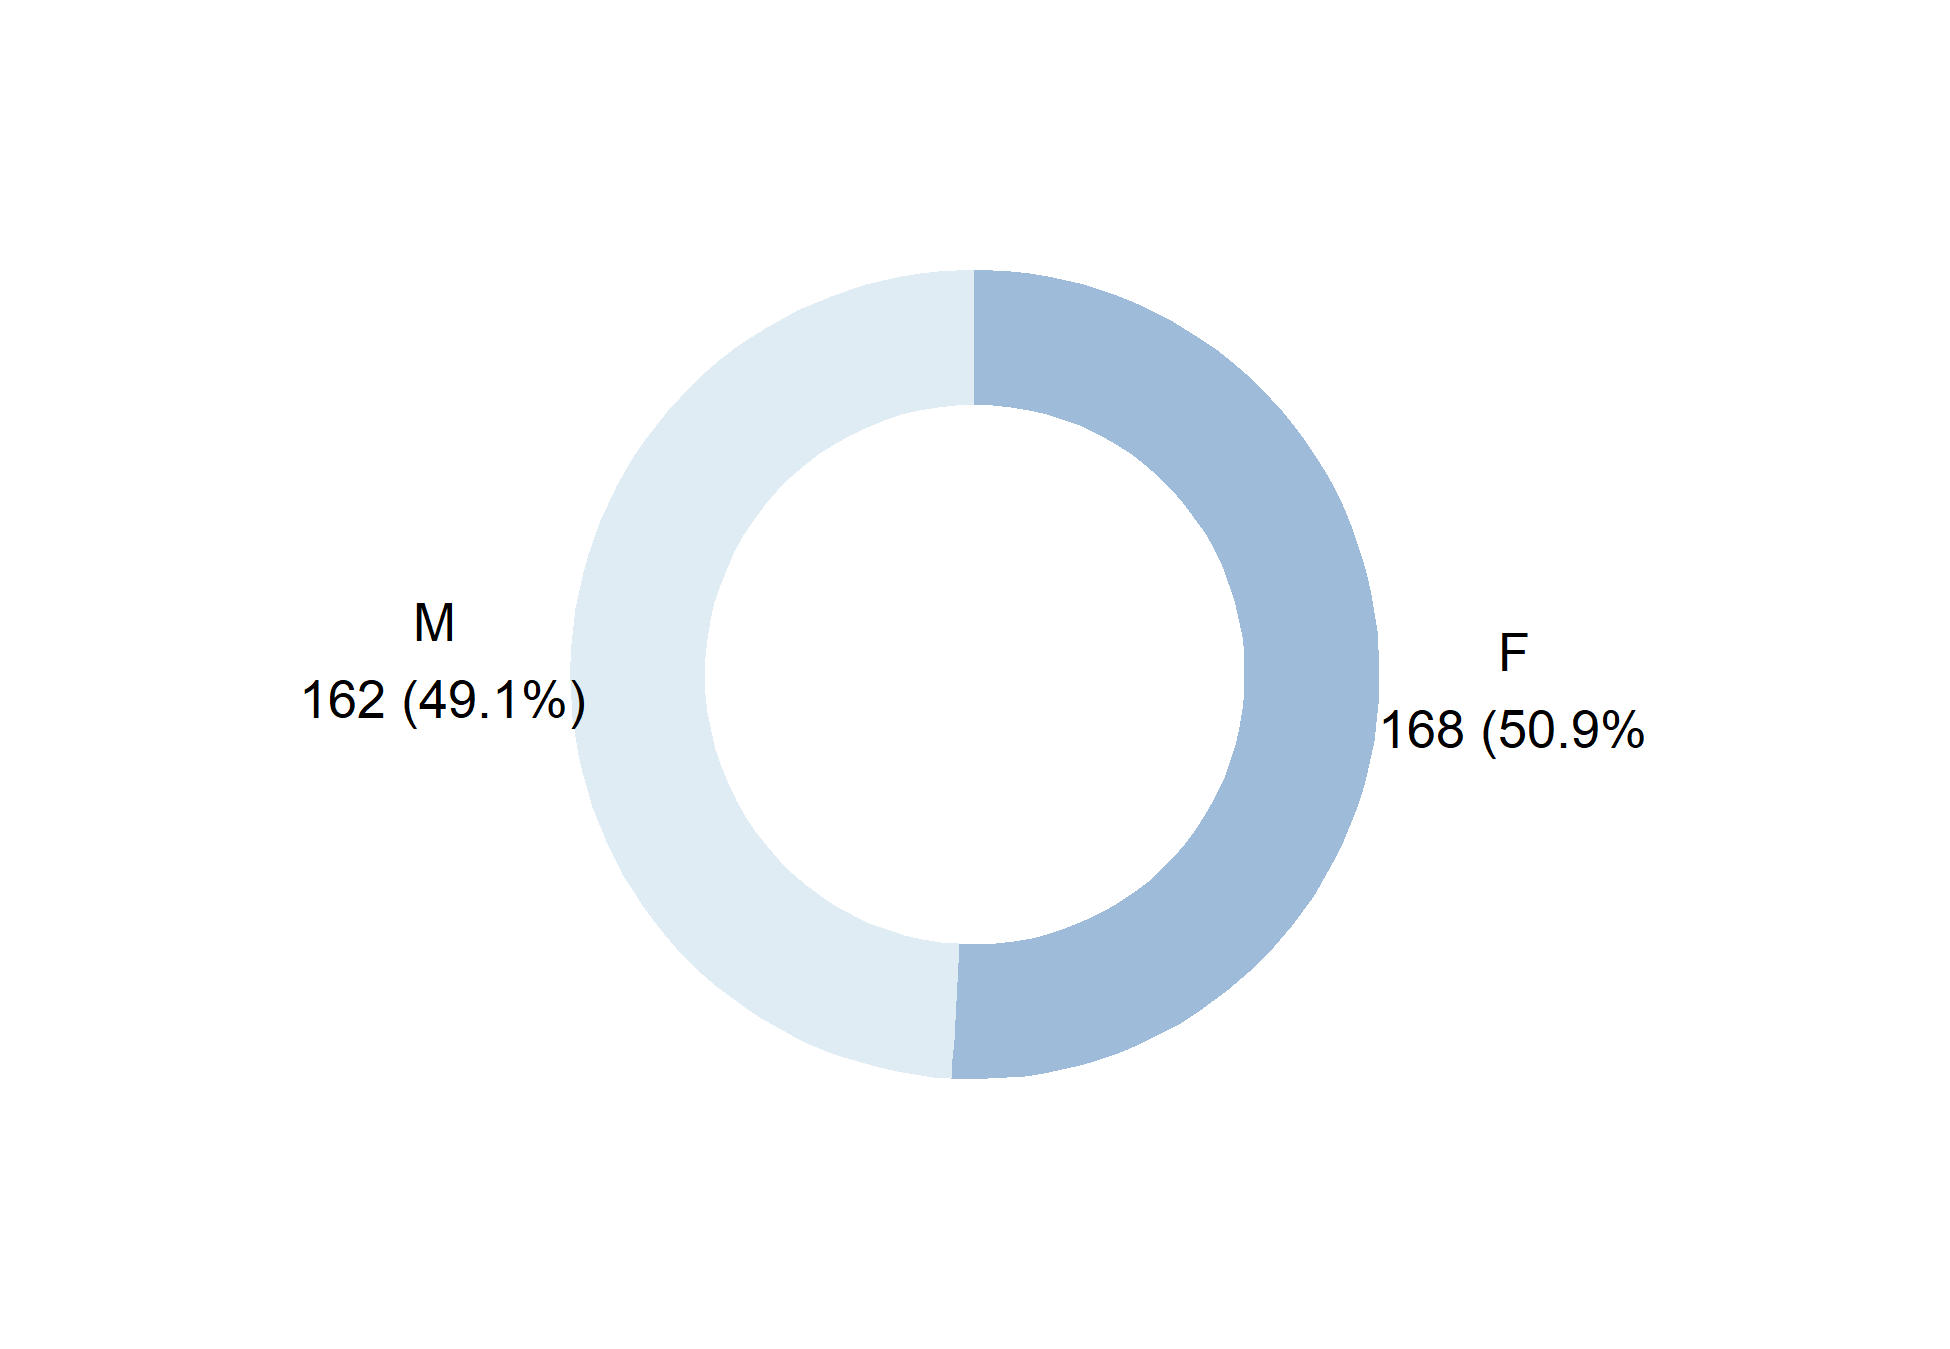
\includegraphics[width=0.7\textwidth]{Imagens/cirurg_SEXO.png}
\end{figure}

\begin{table}[H]

\caption{\label{tab:unnamed-chunk-17}Notificação de acordo com as fases do Procedimento Cirúrgico.}
\centering
\resizebox{\linewidth}{!}{
\begin{tabular}[t]{lrrrrrrrrrrrrr}
\toprule
 & dez/20 & jan/21 & fev/21 & mar/21 & abr/21 & mai/21 & jun/21 & jul/21 & ago/21 & set/21 & out/21 & nov/21 & Total\\
\midrule
\midrule
\textbf{Total} & \textbf{0} & \textbf{0} & \textbf{0} & \textbf{0} & \textbf{0} & \textbf{0} & \textbf{0} & \textbf{0} & \textbf{0} & \textbf{0} & \textbf{0} & \textbf{0} & \textbf{0}\\
\bottomrule
\end{tabular}}
\end{table}

\begin{table}[H]

\caption{\label{tab:unnamed-chunk-18}Incidentes notificados da fase pós-operatória.}
\centering
\begin{tabular}[t]{lr}
\toprule
Pós-operatória & Total\\
\midrule
\midrule
\textbf{Total} & \textbf{0}\\
\bottomrule
\end{tabular}
\end{table}

\begin{table}[H]

\caption{\label{tab:unnamed-chunk-19}Grau de dano das notificações da fase pós-operatória.}
\centering
\begin{tabular}[t]{lr}
\toprule
Grau do Dano & Total\\
\midrule
\midrule
\textbf{Total} & \textbf{0}\\
\bottomrule
\end{tabular}
\end{table}

\subsection{Dados Gerais de Notificação}

\begin{figure}[H]
\caption{Near miss notificados.}
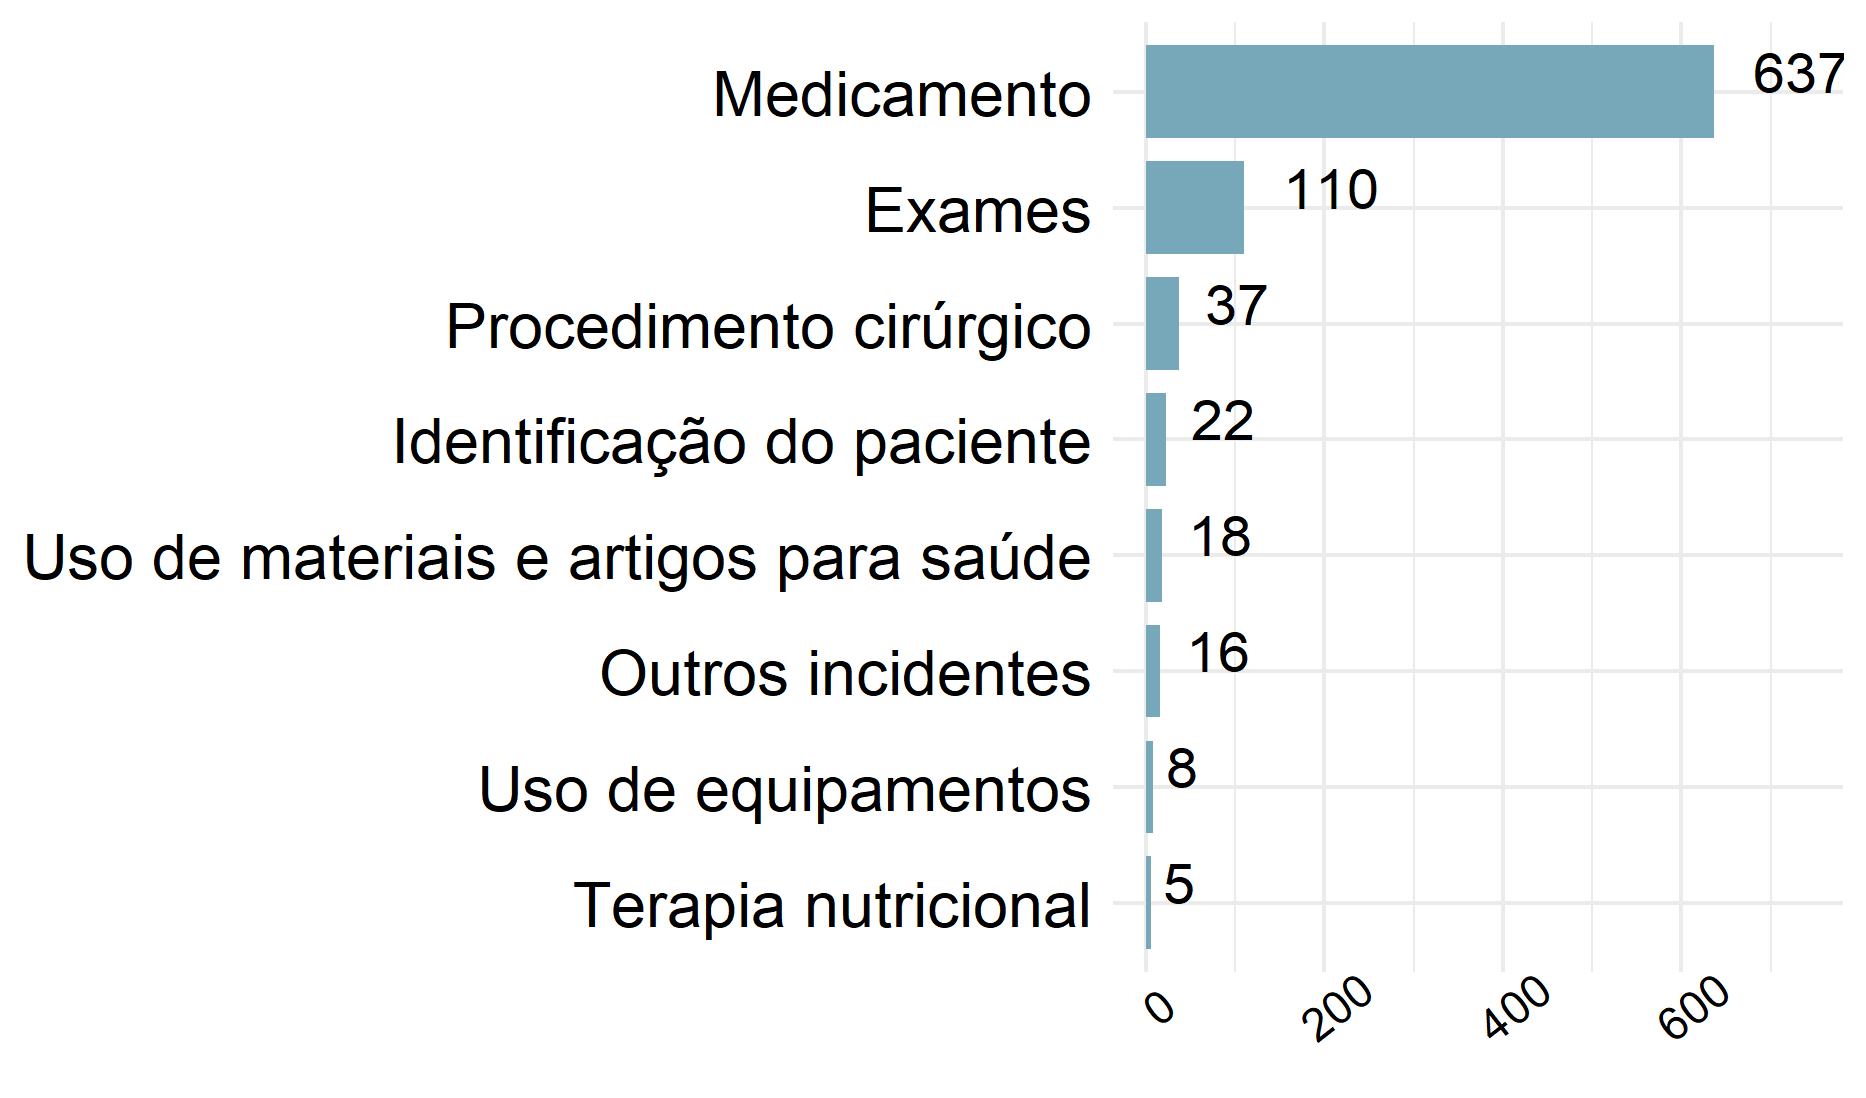
\includegraphics[width=0.7\textwidth]{Imagens/barra_erro.png}
\end{figure}

\begin{figure}[H]
\caption{Incidentes sem dano notificados.}
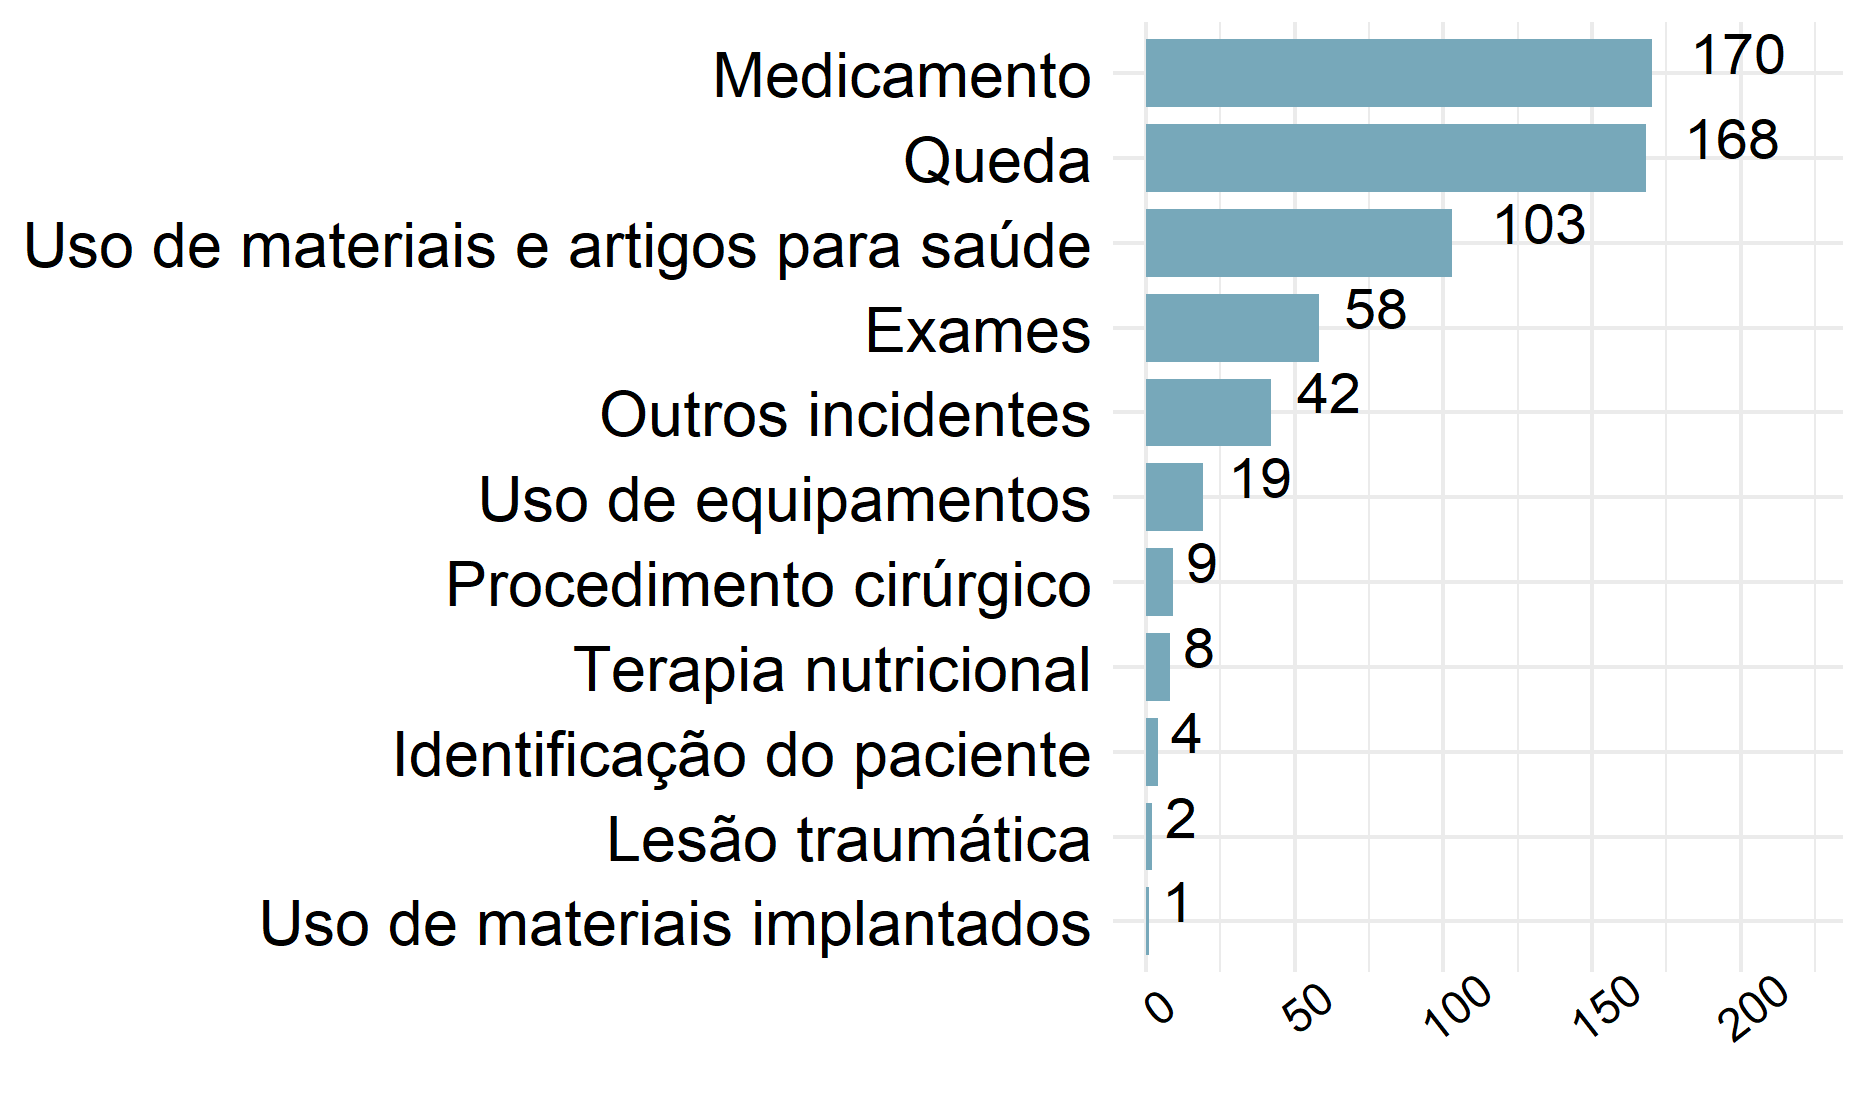
\includegraphics[width=0.7\textwidth]{Imagens/barra_incidente.png}
\end{figure}

\begin{figure}[H]
\caption{Eventos Adversos Notificados.}
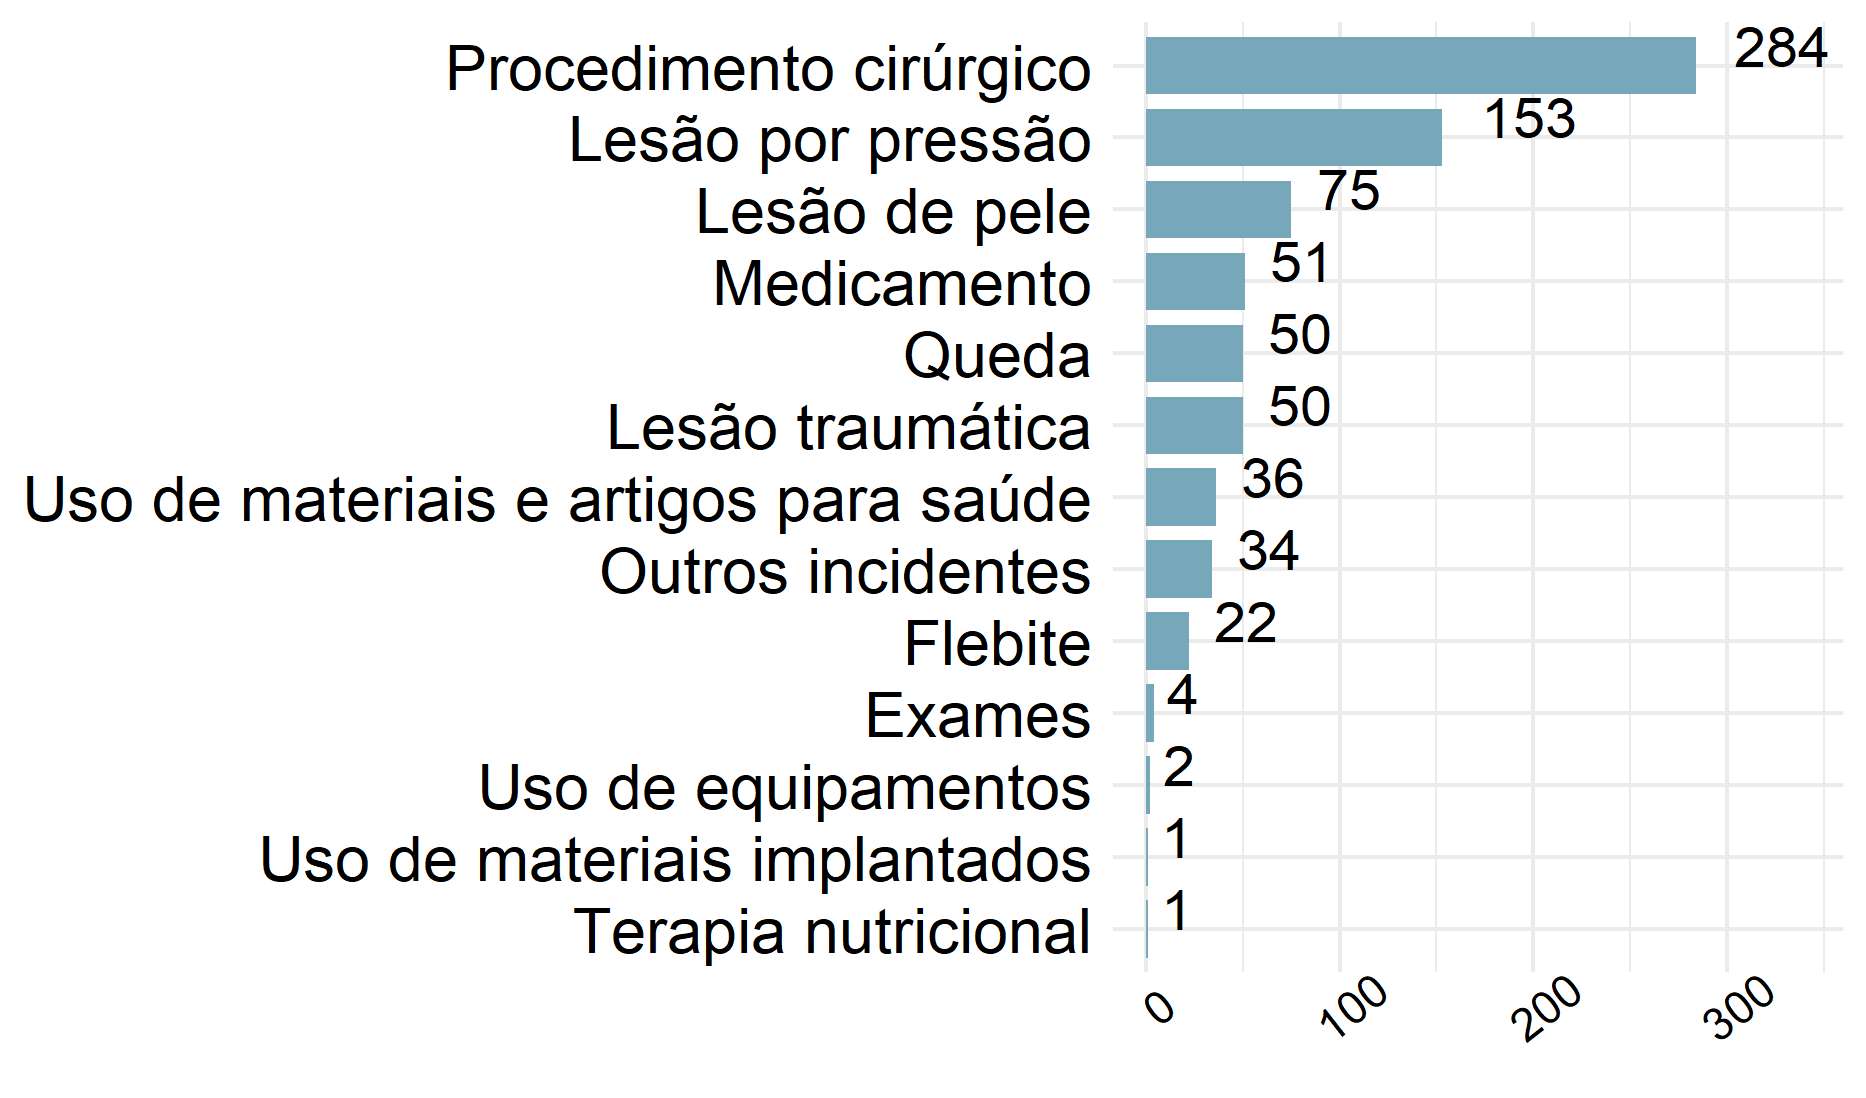
\includegraphics[width=0.7\textwidth]{Imagens/barra_evento.png}
\end{figure}

\end{document}
